\documentclass[twocolumn]{article}

\usepackage{enumerate}
\usepackage{graphicx}
\usepackage[colorlinks=true,linkcolor=blue]{hyperref}
\usepackage[table,xcdraw]{xcolor}
\usepackage[english,spanish]{babel} 
\usepackage{helvet}

\renewcommand{\familydefault}{\sfdefault}

\newenvironment{poliabstract}[1]
   {\renewcommand{\abstractname}{#1}\begin{abstract}}
   {\end{abstract}}

\begin{document}

\title{Herramientas de gestión de pruebas}
\author{Herrera Amezquita,
Derian  \\Paredes Catacora, Randi \\Mejia Rodriguez, Julio\\Marco Garcia Pinto\\Alisson Chino}


\date{06 de Enero del 2021}

\maketitle

\selectlanguage{spanish}
\begin{poliabstract}{Resumen} 
  En el desarrollo del articulo de investigacion expondremos sobre las herramientas de gestión de pruebas 
  se tendra en cuenta los conceptos de las diferentes herramientas que vamos a tratar dando a conocer sus ventajas
   desventajas y demas.
  
\end{poliabstract}

\selectlanguage{english}
\begin{poliabstract}{Abstract} 
  In the development of the research article we will expose about the test management tools
  The concepts of the different tools that we are going to deal with will be taken into account, 
  making their advantages known
  disadvantages and others.
\end{poliabstract}

\section{Introducción}
Las herramientas de gestión de pruebas son aquellas que se utilizan para gestionar la 
información relativa a los «casos de prueba», normalmente los funcionales, para planificar 
actividades de testing, para gestionar los informes resultantes después de pasar dichos test, 
etc.
Es fundamental para cualquier proyecto, salvo que sea muy pequeño, contar con alguna herramienta 
de gestión de pruebas. Hay herramientas que van por separado y otras que integran con 
herramientas complementarias.[1]


\section{Desarrollo}
\subsection{Vs Code}
Visual Studio Code es un editor de código fuente desarrollado por Microsoft para Windows, Linux 
y macOS. Incluye soporte para la depuración, control integrado de Git, resaltado de sintaxis, 
finalización inteligente de código, fragmentos y refactorización de código. También es personalizable, 
por lo que los usuarios pueden cambiar el tema del editor, los atajos de teclado y las preferencias. Es 
gratuito y de código abierto,1aunque la descarga oficial está bajo software privativo e incluye características 
personalizadas por Microsoft.3
Visual Studio Code se basa en Electron, un framework que se utiliza para implementar Chromium y Node.js como 
aplicaciones para escritorio, que se ejecuta en el motor de diseño Blink. Aunque utiliza el framework Electron, 
el software no usa Atom y en su lugar emplea el mismo componente editor (Monaco) utilizado en Visual Studio Team 
Services (anteriormente llamado Visual Studio Online).[2]\\

\includegraphics[width=8cm, height=7cm]{img/vscode.png}
\subsubsection{Historia}

Visual Studio Code fue anunciado el 29 de abril de 2015 por Microsoft en la conferencia Build de 2015. 
Una versión preliminar fue lanzada poco después. El 18 de noviembre de 2015, Visual Studio Code fue lanzado 
bajo la licencia MIT y su código fuente fue publicado en GitHub . También se anunció el soporte de extensión. 
El 14 de abril de 2016, Visual Studio Code graduó la etapa de vista previa pública y se lanzó a la web.[3]\\
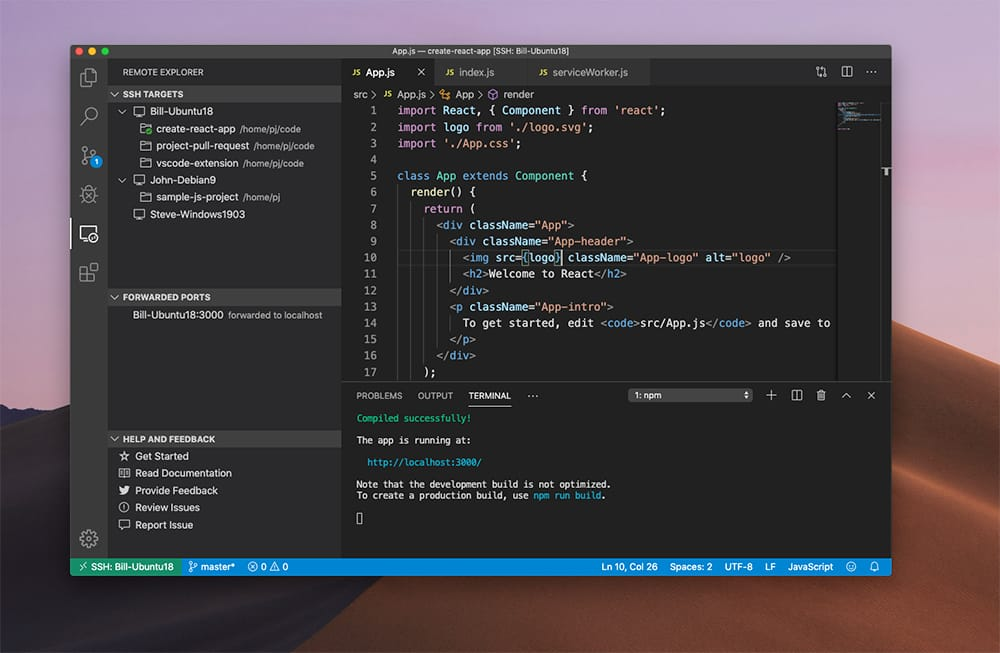
\includegraphics[width=8cm, height=7cm]{img/vscode2.jpg}

\subsubsection{Características}

El código combina la interfaz de usuario optimizada de un editor moderno con asistencia y navegación de código 
enriquecido y una experiencia de depuración integrada, sin la necesidad de un IDE completo. Visual Studio Code, 
cuenta con herramientas de Debug hasta opciones para actualización en tiempo real de nuestro código en la vista 
del navegador y compilación en vivo de los lenguajes que lo requieran (por ejemplo en el caso de SASS a CSS). Además 
de las extensiones, tendremos la posibilidad de optar por otros themes o bien configurarlo a nuestro gusto. Para 
modificar el esquema de colores y los iconos.[4]\\

\subsubsection{Ventajas}

  1. Se puede utilizar como lenguajes de programación.\\
  2. Visual Studio Code es una herramienta que tiene soporte nativo para gran variedad de lenguajes, entre ellos podemos destacar los principales del desarrollo Web: HTML, CSS, y JavaScript, entre otros.\\
  3. Posibilidad de configurar la interfaz a nuestro gusto. De esta forma, podremos tener más de un código visible al mismo tiempo, las carpetas de nuestro proyecto y también acceso a la terminal o un detalle de problemas, entre otras posibilidades.\\
  4. Existencia de una amplísima gama de temas o estilos visuales para Visual Studio Code, que hacen el trabajo con el software más agradable a la vista.\\
  5. Goza de un soporte técnico formidable pues debido a su frecuente uso por la comunidad de desarrolladores, se puede encontrar fácilmente documentación y ayuda en foros y sitios relacionados.[5]\\

   
\subsection{MiKTeX}
\subsubsection{Latex}
LaTeX es un sistema de composición de textos, orientado especialmente a la creación de libros, documentos científicos y técnicos que contengan fórmulas matemáticas.

LaTeX está formado por un gran conjunto de macros de TeX, escrito por Leslie Lamport en 1984, con la intención de facilitar el uso del lenguaje de composición tipográfica, TeX, creado por Donald Knuth. Es muy utilizado para la composición de artículos académicos, tesis y libros técnicos, dado que la calidad tipográfica de los documentos realizados con LaTeX es comparable a la de una editorial científica de primera línea.

\includegraphics[width=8cm, height=7cm]{img/latex.png}

\subsubsection{¿Qué es MiKTeXo}
ores de bases de datos, los administradores de bases de datos y los administradores de sistemas. Azure Data Studio genera un aumento en su productividad con fragmentos de código inteligente, finalización de palabras clave, IntelliSense, integración de control de fuente, la capacidad de ver y guardar resultados en formato CSV, Excel, JSON y la capacidad de organizar y administrar las conexiones de base de datos favoritas, etc. La versión de Azure Data Studio se lanzó en Noviembre de 2017.[6]

\includegraphics[width=8cm, height=7cm]{img/mik.png}

\subsubsection{Características}
Las principales características de MiKTeX son las siguientes:\\

Es libre y fácil de instalar.\\
Incluye más de 800 paquetes con tipografías, macros, etc.\\
Tiene un visor propio de archivos dvi denominado Yap.\\
Su código es abierto.\\
Posee compiladores TeX y LaTeX, convertidores para generar archivos PostScript (.ps), .pdf, .html, etc.; y herramientas para generar bibliografías e índices.\\
Posee tres formas de instalación: pequeña, mediana y completa.\\


\section{Bibliografía}

\begin{thebibliography}{X}
  
  
  \bibitem{Baz} \textsc{} ,
  \textit{}(2021)Análisis y comparativa de herramientas de gestión de pruebas de uso gratuito, Javier Garzas de \url{https://www.javiergarzas.com/2013/10/herramientas-de-gestion-de-pruebas.html#:~:text=Las%20herramientas%20de%20gesti%C3%B3n%20de,de%20pasar%20dichos%20test%2C%20etc.}
  
  
  \bibitem{Baz} \textsc{Lardinois, Frederic } ,
  \textit{}(2015),Microsoft Launches Visual Studio Code, A Free Cross-Platform Code Editor For OS X, Linux And Windows». TechCrunch.\url{https://www.cs.princeton.edu/courses/archive/spring07/cos424/lectures/li-guest-lecture.pdf}


  \bibitem{Baz} \textsc{Ecured} ,
  \textit{}(2020)Visual Studio Code\url{https://www.ecured.cu/Visual_Studio_Code}
  
  \bibitem{Baz} \textsc{Damian de Luque} ,
  \textit{}(2019)Visual Studio Code: características principales\url{https://damiandeluca.com.ar/visual-studio-code-caracteristicas-principales}

  \bibitem{Baz} \textsc{Ecured} ,
  \textit{}(2020)Visual Studio Code\url{https://www.ecured.cu/Visual_Studio_Code}

  \bibitem{Baz} \textsc{SQLShack} ,
    \textit{}(2019)Azure Data Studio para Windows\url{https://www.sqlshack.com/es/como-poder-instalar-y-configurar-azure-data-studio-para-windows/#:~:text=Azure%20Data%20Studio%20es%20una,y%20Azure%20SQL%20Data%20Warehouse.}
  
    \bibitem{Baz} \textsc{Sergio Luján Mora} ,
    \textit{}(2019)Herramientas para la investigación\url{http://desarrolloweb.dlsi.ua.es/cursos/2015/herramientas-investigacion/que-es-latex}


\end{thebibliography}


\end{document}